% created on 12/05/2020
% @author : ebazan

\chapter{Color image texture analysis based on Gabor features}\label{ch:complex_spectral_image_decomposition}
\section*{Résumé}
\noindent Dans ce chapitre, nous présentons la décomposition spectrale d'une image couleur avec l'aide du filtre de Gabor. Nous utilisons la théorie sur les fonctions de Gabor développée dans le Chapitre \ref{ch:image_spectral_decomposition} pour extraire les caractéristiques de texture locale d'une image en couleurs. La stratégie principale consiste à transformer l'image d'entrée d'un espace couleur réel à trois canaux en une représentation couleur complexe à deux canaux. Ensuite, nous utilisons une banque de filtres Gabor sur chaque canal de l'image pour extraire les informations de texture générées par les variations de couleur et d'illumination de l'image.

\section*{Abstract}
\noindent In this chapter we present the spectral decomposition of a color image by means of the Gabor filter. We use the theory about Gabor functions developed in Chapter \ref{ch:image_spectral_decomposition} to extract local texture features of a color image. The main strategy consist on transforming the input image from a three-channel real color space into a two-channel complex color representation. Then, we use a bank of Gabor filters on each channel of the image to extract the texture information generated by the variations of color and illumination in the image.

\section{Introduction}

Gabor filters have long been used for analyzing textures and extracting corresponding image features. Its adaptability and customization depending on the application and the relationship with the human visual system \citep{Daugman:JOSA:1985a}, have made this technique one of the most relevant for the analysis of textures in an image.

The use of Gabor filters for image texture analysis is highly dependent on the final application. Some of the most recognized works in the literature date back to the late 90s, where this technique was a hot research topic for image texture analysis. However, regarding the works present in the literature, we can make a clear separation of the methods taking into account the nature of the extracted features. The first group uses Gabor filters to extract a global texture descriptor (Gabor signature). Generally this strategy is suitable for applications where the images contain homogeneous textures and it is sought to make the the classification of images or an image retrieval system based on the content, as we can see in Chapter \ref{ch:similarity_measures}. The second group is characterized by using Gabor filters to obtain local texture features present in an image. Such a strategy is suitable for image segmentation tasks. In this Chapter we address in a detailed and comprehensive way the second case, delving into the spectral decomposition of color images to obtain texture features generated by the changes in illumination and / or color.

In both aforementioned cases of use, we take advantage of the Gabor function's dual-domain (spatial and frequency) representation capability to create a bank of filters $\mathcal{G}=\{g_{f, \theta}(x, y) \}$ that works at different central frequencies $f$ (scales) and orientations $\theta$ to obtain the spectral decomposition of an input image $I(x, y)$ through the convolution operation of each of the filters. 

\begin{equation}\label{eq:gabor_responses}
    r_{f, \theta}(x,y) = I(x, y) \ast g_{f, \theta}(x,y)
\end{equation}

As we know, due to the complex form of Gabor's filters \ref{eq:gabor_function_2d_spacefreq_bank} defined in Chapter \ref{ch:image_spectral_decomposition}, the response of the filter $r_{f,\theta}(x, y)$ will have, in the same way as the filter, a real part and an imaginary part, here denoted as $\Re{(\cdot)}$ and $\Im{(\cdot)}$, respectively.

The linear transformation of an image using Eq. \eqref{eq:gabor_responses}, produces considerable information about the textures present in the image. The efficient manipulation of this information is the basis for the extraction of appropriate (local or global) texture features. Although the convolution of the image by a filter bank is a common denominator in techniques based on signal processing, in the literature we can find various schemes to create more separable texture features (see Figure \ref{fig:general_pipeline_gabor_feature_extraction}). In general, these methods vary in the type of output they use to measure the textural information of the image and the post-processing performed

The possible filter responses to measure the texture information are: 

\begin{enumerate}
    \item Amplitude of the response (magnitude or Gabor energy) \citep{Bovik.Clark.ea:TPAMI:1990}.
        \begin{equation}\label{eq:gabor_magnitude}
            |r_{f, \theta}(x,y)| = \sqrt{\Re{(r_{f, \theta}(x, y))}^2 + \Im{(r_{f, \theta}(x, y))}^2}
        \end{equation}
    \item Phase of the response \citep{Palm.Lehmann:MGV:2002}.
    \begin{equation}\label{eq:gabor_phase}
            \arg(r_{f, \theta}(x,y)) = \arctan2{\left(\frac{\Im{(r_{f, \theta}(x, y))}}{\Re{(r_{f, \theta}(x, y))}}\right)}
        \end{equation}
    \item Real component of the response \citep{Jain.Farrokhnia:IJPR:1991}.
    \begin{equation}\label{eq:gabor_real_part}
            \Re{(r_{f, \theta}(x, y))}
        \end{equation}
    \item Square amplitude of the response (Gabor local power spectrum) \citep{Grigorescu.Petkov.ea:TIP:2002}.
    \begin{equation}\label{eq:gabor_power}
            |r_{f, \theta}(x,y)|^2 = \Re{(r_{f, \theta}(x, y))}^2 + \Im{(r_{f, \theta}(x, y))}^2
        \end{equation}
\end{enumerate}
whereas the most common post-processing techniques for the filter outputs consists on a non-linear transformation followed by smoothing using a rectangular or Gaussian window \citep{Randen.Husoy:TPAMI:1999}, \citep{Clausi.EdJernigan:JPR:2000}. 
The application of non-linearity favors the activation of the textured areas in the images, while the smoothing favors the location of the energy obtained with the filter, avoiding the loss of information from the natural contours of the image. Figure \ref{fig:general_pipeline_gabor_feature_extraction} illustrate the stages (boxes with black continuous lining) and the input/outputs (boxes with black dotted lining) of the aforementioned scheme for the extraction of Gabor-based texture features.

\begin{figure}[!ht]
	\centering
	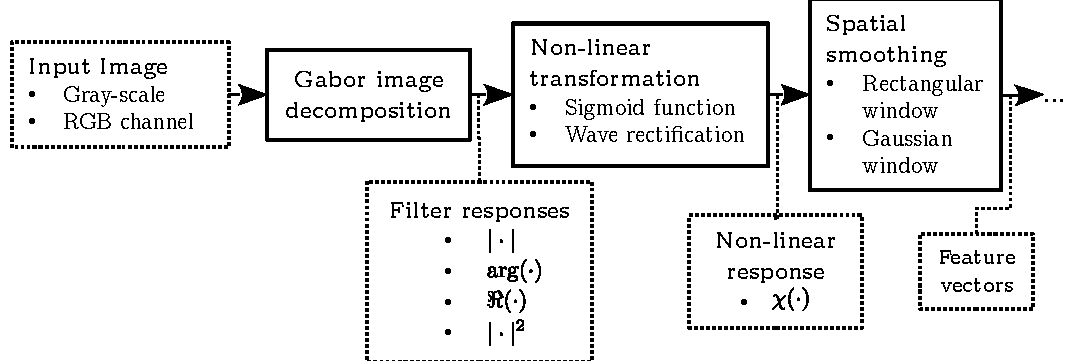
\includegraphics[width=\textwidth]{general_pipeline_gabor_feature_extraction}
	\caption{General pipeline for extraction of texture features using the Gabor filters.}\label{fig:general_pipeline_gabor_feature_extraction}
\end{figure}

The model that we propose in this chapter follows the stages of figure \ref{fig:general_pipeline_gabor_feature_extraction} with some modifications to obtain the local features of a color image. First, we transform the input image from RGB space into a two-channel space (one real and one complex) that represent the luminance and chrominance information of the image. After that, we use the bank of optimized filters from the previous chapter for the decomposition of each channel of the image. Later, we replace the non-linear transformation with a morphological opening to highlight the amplitude of the filter responses and then apply an adaptive Gaussian smoothing. Following this flow, we obtain a spectral decomposition of the image that takes into account the textures generated by changes in lighting but also by those generated by color changes. The figure \ref{fig:proposed_pipeline_gabor_feature_extraction} shows the diagram with the stages that we follow for the extraction of local features.

\begin{figure}[!ht]
	\centering
	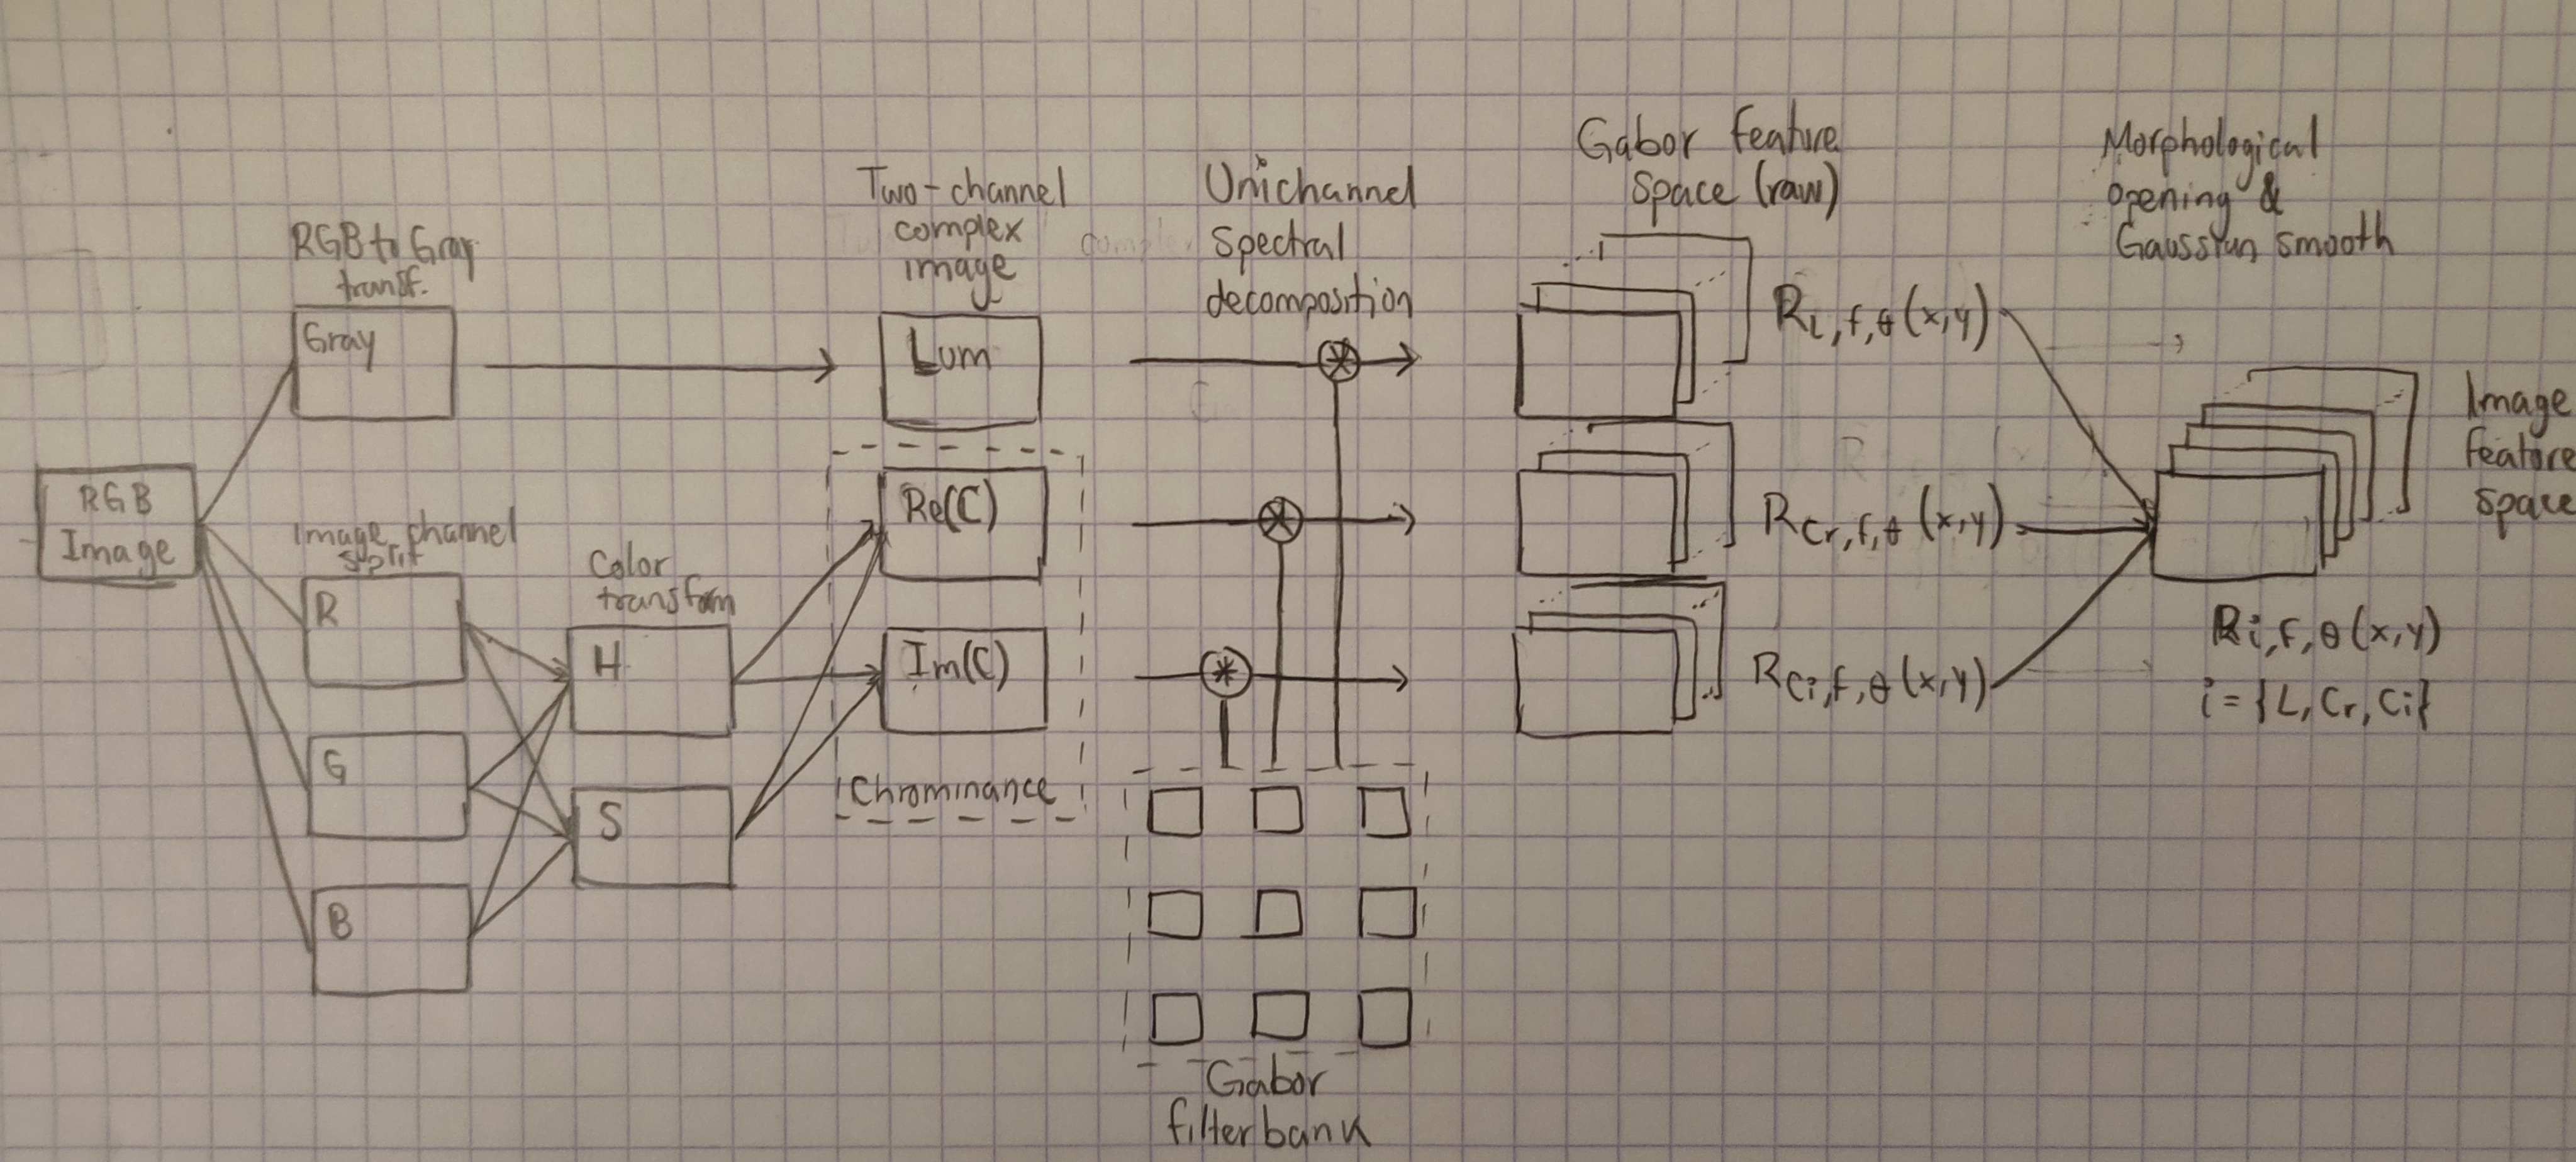
\includegraphics[width=\textwidth]{pipeline_gabor_color_feature_extraction}
	\caption{Proposed methodology for the computation of Gabor features in color images.}\label{fig:proposed_pipeline_gabor_feature_extraction}
\end{figure}


\subsection{Texture features for color images}
Most of the research work on texture has been done in the field of gray-scale images with homogeneous textures. In consequence, the first and simplest way to obtain texture features from color images is to transform it into a gray-scale image. This strategy favors the acceleration of feature calculation because we work with scalar values instead of vectors. However, despite the good results in images with homogeneous gray-scale textures, reducing channels for a natural color image with non-homogeneous textures does not ensure the generation of representative texture features for a colored real-world image containing non-homogeneous textures. This idea is based on the relationship principle that have the texture and color in a real image and how we use this information \citep{Maenpaa.Pietikainen:PR:2004}. Although certain works in the literature on the analysis of homogeneous color textures consider that the variation of the spatial structure (texture) and the color distribution in the image are independent cues \citep{Permuter.Francos.ea:PR:2006}, we differ from this point of view and we consider that color and texture information in a image are a joint phenomenon.

A popular technique based on the $RGB$ primary color space consist in applying the Gabor decomposition in each image channel to obtain a vector of unichromatic features. The filter output represents the features of each color channel independently, so this strategy does not involve the correlation between $RGB$ band colors. This might be corrected using the opponent color model based on the human color vision theory \citep{Jain.Healey:TIP:1998}. In this case each unichromatic feature vector ($RGB$-feature) is multiplied and normalized by the feature vector of its opponent color to include the correlation between color channels, which implies an extra post-processing step in the extraction pipeline of features.

One way to avoid the post-processing stage is to first transform the color image in a color space that handles the coupling between the color channels rather than separating them as components of the color space, and then performing the Gabor decomposition. One possible option for the color representation is the quaternion framework \citep{Sangwine.Ell:VISP:2000}. This encodes the color value of each pixel in a pure quaternion, where the real component is set to zero and the three imaginary components represent the color band such as $I(x, y) = R (x, y) i + G (x, y) j + B (x, y) k $. This 3-component vector representation yields a system which has well-defined mathematical operations, such as Quaternion Fourier Transform, which makes possible the Gabor image decomposition by means of the Quaternion Gabor Filters (QBF) \citep{Subakan.Vemuri:EMMCVPR:2009}. However, when using quaternion values, the non-existing commutativity has to be taken into account, in addition, the QGF does not support any physic interpretation of what is measured.

For example, consider a texture image in the $RGB$ color space, where its gray-scale transformation represents the levels of red, green, and blue at a single luminance value $Y$ obtained with conversion equation of the ITU Rec. 709 \citep{Artusi.Banterle.ea:Book:2016}.

\begin{equation}\label{eq:color2gray_formula}
    L = 0.2126 R + 0.7152 G + 0.00722 B
\end{equation}
 
Although there is some texture information in the color input image, in the case of isoluminant colors or colors with the same luminance value, the transformation $L$ leads to a minimization or lost, in the worst case, of textures generated by the color changes. This is because the non-homogeneous textures in a color image are not only generated by lighting variations, but also by variations in chromaticity. Moreover, the real world scenes are in color and contain non-homogeneous textures.

%\textit{Idea to develope:} Illustrate the effect of compute unichrome features in the gray-scale and the RGB space for a color image.

In both cases, the choice of a pertinent color space for the characterization of the texture is necessary \citep{Qazi.Alata.ea:PR:2011}. We can represent the image in a primary color space such as the $RGB$, in a Luminance-Chrominance based color space such as the $L^*a^*b^*$ or the $LUV$, or in a perceptual color space such as the $HSV$ or the $HLS$ \citep{Hanbury:IA:2003}. 





\section{Two-channel complex image representation}

From the previous section, it is clear that the luminance information is a cue in obtaining texture features, however, the chrominance also plays an important role. We can obtain this information using the two-complex channels form. This representation contains the pure luminance $L^*$ values in a real channel while the chrominance $C$ is contained in a complex channel. This complex channel can be obtained from the components of the $L^*a^*b^*$ or the components of $HSV$ / $HLS$ color spaces prior to a transformation of the image from the $RGB$ space.

Thus, the complex chrominance channel in its exponential form is defined as  

\begin{equation}\label{eq:chrominance_hsv}
    C(x,y) = S(x,y) e^{iH(x,y)}
\end{equation}
where $H$ is the hue and $S$ is the saturation value obtained after the $RGB$ to $HLS$ transformation. While the combined chrominance function for $L^*a^*b^*$ is defined as

\begin{equation}\label{eq:chrominance_lab}
    C(x,y) = a^*(x,y) + ib^*(x,y)
\end{equation}
where $a^*$ and $b^*$ are two chroma variables obtained from $RGB$ to $L^*a^*b^*$ transformation. 

We obtain a complex representation of chrominance content of the image whose spectrum is interesting to analyze in order to characterize the spatial variations of the chromatic part of the image. 

\section{Spectral decomposition of color images}

The representation in two channels, one real and the other complex, of a color image allows us to separate the intervention of luminance and colors in the generation of textures in the image. To help visualize such a joint phenomenon, we create a synthetic image. Figure \ref{fig:synthetic_color_texture_image} contains seven different regions with spatial variations generated by the combination of different colors. For comprehension purposes, we use colors that are easily identified in the $RGB$ space (primary colors) or in the $HSV$ space (perceptual colors).

\begin{figure}
    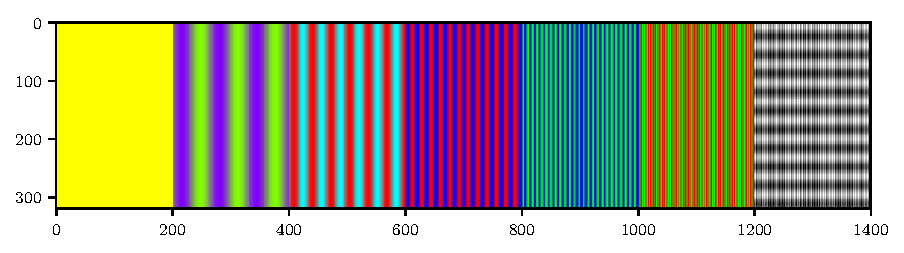
\includegraphics[width=\textwidth]{synthetic_image_color_texture.pdf}
\caption{Synthetic color textured image.}\label{fig:synthetic_color_texture_image}
\end{figure}

\begin{table}[h!]
\resizebox{\textwidth}{!}{%
\begin{tabular}{c|ccccccc}
                    & \multicolumn{7}{c}{\textbf{Region}}                                                                                                                                                                          \\ \hline
\textbf{}           & 1                  & 2                   & 3                   & 4                   & 5                   & 6                   & 7                                                              \\ \hline
\textbf{Color 1}    &                    &                     &                     &                     &                     &                     &                                                                \\
\textit{Name}       & Yellow             & Purple              & Red                 & Red                 & Blue                & Green               & Black                                                          \\
\textit{RGB values} & {[}255, 255, 0{]}  & {[}128, 0, 255{]}   & {[}255, 0, 0{]}     & {[}255, 0, 0{]}     & {[}0, 0, 255{]}     & {[}0, 255, 0{]}     & {[}0, 0, 0{]}                                                  \\
\textit{HSV values} & {[}60, 100, 100{]} & {[}270, 100, 100{]} & {[}0, 100, 100{]}   & {[}0, 100, 100{]}   & {[}240, 100, 100{]} & {[}120, 100, 100{]} & {[}0, 0, 0{]}                                                  \\ \hline
\textbf{Color 2}    &                    &                     &                     &                     &                     &                     &                                                                \\
\textit{Name}       & -                  & Green lime          & Cyan                & Blue                & Green               & Red                 & White                                                          \\
\textit{RGB values} & -                  & {[}128, 255, 0{]}   & {[}0, 255, 255{]}   & {[}0, 0, 255{]}     & {[}0, 255, 0{]}     & {[}255, 0, 0{]}     & {[}255, 255, 255{]}                                            \\
\textit{HSV values} & -                  & {[}90, 100, 100{]}  & {[}180, 100, 100{]} & {[}240, 100, 100{]} & {[}120, 100, 100{]} & {[}0, 100, 100{]}   & {[}0, 0, 100{]}                                                \\ \hline
\textbf{Texture}    &                    &                     &                     &                     &                     &                     &                                                                \\
\textit{Freq.}      & -                  & $1/64$              & $1/32$              & $1/16$              & $1/8$               & $1/4$               & \begin{tabular}[c]{@{}c@{}}$1/8$\\ $1/32$\end{tabular}         \\
\textit{Angle}      & -                  & $90^\circ$          & $90^\circ$          & $90^\circ$          & $90^\circ$          & $90^\circ$          & \begin{tabular}[c]{@{}c@{}}$0^\circ$\\ $90^\circ$\end{tabular}
\end{tabular}}
\caption{Specifications of color and texture of the areas of the synthetic study image.}\label{tab:synthetic_image_components}
\end{table}

\begin{figure}[h!]
	\centering
    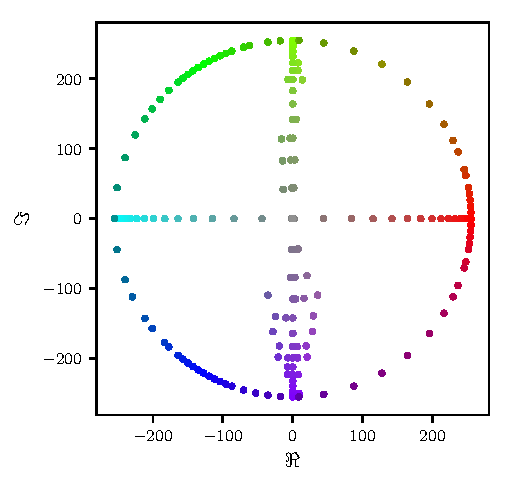
\includegraphics{color_complex_plane.pdf}
\caption{Two-channel color complex plane.}\label{fig:color_complex_plane}
\end{figure}


\subsection{Synthetic image description}

The textures of the image are formed by 2-d sinusoidal modulations at a certain frequency. These modulations change the colors of the regions generating a texture of oriented lines. The regions of the synthetic image have the following color and texture characteristics.

\paragraph{Region 1. Textureless zone:}
This region does not contain spatial variations, i.e., it has only a solid color. The color of the region is yellow.

\paragraph{Region 2. Lowest frequency textured zone with colors on the imaginary plane:}
This region is described by the horizontal texture generated by the variations between purple and green lime. Such colors are found in the imaginary axis of the $HSV$ space. The colors change every 64 pixels.

\paragraph{Region 3. Textured zone with colors on the real plane:}
This region contains an horizontal texture generated by the variations between red and cyan. Such colors are found in the real axis of the $HSV$ space. The colors change every 32 pixels.

\paragraph{Region 4. Textured zone with two primary colors:}
The horizontal texture of this region is generated by the variations between red and blue. The colors change every 16 pixels. 

\paragraph{Region 5. Textured zone with two primary colors:}
The horizontal texture of this region is generated by the variations between blue and green. The colors change every 8 pixels. 

\paragraph{Region 6. Textured zone with two primary colors:}
The horizontal texture of this region is generated by the variations between green and red. The colors change every 4 pixels.

\paragraph{Region 7. Colorless mixed textures zone:}
This region contains two textures, both of them formed by the variations between black and white, i.e., there is no color information. Moreover, the textures change in frequency and orientation; the pixes of the horizontal one change of color every 4 pixels, while the pixel values of the vertical one changes every 32 pixels.

The colors and frequency of each zone are summarized in Table \ref{tab:synthetic_image_components}. In it, we expose the $RGB$ and $HSV$ values of the texture-forming colors as well as the frequency and orientation of each section.

%\begin{table}[h!]
%\resizebox{\textwidth}{!}{%
%\begin{tabular}{c|c|c|c|c|c|c|c|c|}
%\cline{2-9}
%\textbf{}                                & \multicolumn{6}{c|}{\textbf{Colors}}                                                                                                                                        & \multicolumn{2}{c|}{\multirow{2}{*}{\textbf{Texture}}} \\ \cline{2-7}
%                                         & \multicolumn{3}{c|}{\textbf{Color 1}}                                            & \multicolumn{3}{c|}{\textbf{Color 2}}                                                    & \multicolumn{2}{c|}{}                                  \\ \hline
%\multicolumn{1}{|c|}{\textbf{Zone}}      & \textbf{Name}          & \textbf{$RGB$ values}      & \textbf{$HSV$ values}      & \textbf{Name}          & \textbf{$RGB$ values}            & \textbf{$HSV$ values}        & \textbf{Freq.}             & \textbf{Angle}            \\ \hline
%\multicolumn{1}{|c|}{1}                  & Yellow                 & $[255,255,0]$              & $[60,100,100]$             & n/a                    & n/a                              & n/a                          & n/a                        & $90^\circ$                \\ \hline
%\multicolumn{1}{|c|}{2}                  & Purple                 & $[128, 0, 255]$            & $[270,100,100]$            & Green lime             & $[128, 255, 0]$                  & $[90,100,100]$               & $\frac{1}{64}$             & $90^\circ$                \\ \hline
%\multicolumn{1}{|c|}{3}                  & Red                    & $[255,0,0]$                & $[0,100,100]$              & Cyan                   & $[0,255,255]$                    & $[180,100,100]$              & $\frac{1}{32}$             & $90^\circ$                \\ \hline
%\multicolumn{1}{|c|}{4}                  & Red                    & $[255,0,0]$                & $[0,100,100]$              & Blue                   & $[0,0,255]$                      & $[240,100,100]$              & $\frac{1}{16}$             & $90^\circ$                \\ \hline
%\multicolumn{1}{|c|}{5}                  & Blue                   & $[0,0,255]$                & $[240,100,100]$            & Green                  & $[0,255,0]$                      & $[120,100,100]$              & $\frac{1}{8}$              & $90^\circ$                \\ \hline
%\multicolumn{1}{|c|}{6}                  & Green                  & $[0,255,0]$                & $[120,100,100]$            & Red                    & $[255,0,0]$                      & $[0,100,100]$                & $\frac{1}{4}$              & $90^\circ$                \\ \hline
%\multicolumn{1}{|c|}{\multirow{2}{*}{7}} & \multirow{2}{*}{Black} & \multirow{2}{*}{$[0,0,0]$} & \multirow{2}{*}{$[0,0,0]$} & \multirow{2}{*}{White} & \multirow{2}{*}{$[255,255,255]$} & \multirow{2}{*}{$[0,0,100]$} & $\frac{1}{4}$              & $90^\circ$                \\ \cline{8-9} 
%\multicolumn{1}{|c|}{}                   &                        &                            &                            &                        &                                  &                              & $\frac{1}{32}$             & $0^\circ$                 \\ \hline
%\end{tabular}}
%\caption{Specifications of color and texture of the areas of the synthetic study image.}\label{tab:synthetic_image_components}
%\end{table}

The choice of texture forming colors comes from the interest in visualizing the color spectrum of the image in a more representative way. Throughout this work, we will use the representation of color in two-complex channels from the $HSV$ color space given by Eq. \eqref{eq:chrominance_hsv}.

Considering that the colors of the input image are initially expressed in spectral light primaries $RGB$, if we look at the colors in the $HSV$ space on the complex plane (see Fig. \ref{fig:color_complex_plane}), a pure value of hue ($H$) equivalent to a full saturation corresponds to the ratio of the dominant wavelength to other wavelengths in color. The saturation ($S$) or chroma defines the brilliance and intensity of a color; it refers to the dominance of hue in the color. Finally, the value ($V$) refers to the lightness or darkness of a color; it indicates the quantity of light reflected.


Since for the representation in two complex channels the value $V$ of each pixel is not necessary, we can plot the pixel values of hue $H$ (in degrees) and saturation $S$ (normalized between $0$ and $255$) in the complex 2-d plane shown in the Figure \ref{fig:color_complex_plane}. This representation completes the description of our synthetic test image showing the variation between colors that generate textures. We can see in Figure \ref{fig:color_complex_plane} the transition between the $RGB$ primary colors at $0^\circ$, $120^\circ$ and $240^\circ$ respectively; the transition between purple and lime green on the imaginary axis with a hue of $90^\circ$ and $270^\circ$ respectively; the transition between red at $0^\circ$ and cyan at $180^\circ$ passing through the real axis of the plane and finally the yellow color with a hue value of $60^\circ$ in the chroma circle.

Now that the colors are represented in the two complex channels, it only remains to represent the spatial variations produced by the intensity changes. Generally when the complex representation of two channels is used, the lighting is not taken into account or, the $L^*$ channels of the $L^*a^*b^*$ space or V of the $HSV$ space take on this role. In our case, we use the transformation of the image in $RGB$ to the gray-scale following the Eq. \eqref{eq:color2gray_formula}. Then, if we plot these three channels separately ($L(x,y)$, $\Re(C(x,y))$, $\Im(C(x,y))$), Figure \ref{fig:synthetic_image_three_channel_decomposition}, and consider a horizontal line through the synthetic image, Figure \ref{fig:horizontal_line_three_channel_decomposition}, we can observe the variations generated by changes in color or changes in intensity. For example, taking the area without texture (region 1), the horizontal line between pixels 0 and 200 remains constant in all three channels due to the absence of texture. Observing region 2, which corresponds to the low frequency texture formed by the colors at 90 and 180 in the chroma circle, we can see that the variations are only present in the imaginary channel of chrominance $\Im(C(x,y))$; while for the last region (colorless mixed textures zone), we can see that the variations are only present in the channel that describes the luminance $L(x,y)$.

\begin{figure}
\centering
    \subcaptionbox{\label{fig:synthetic_image_three_channel_decomposition}}{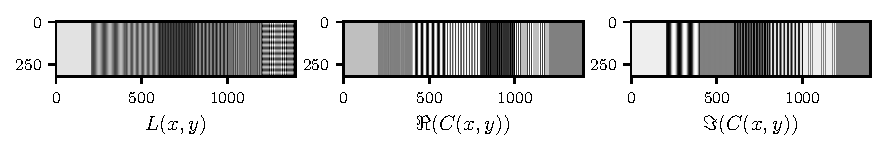
\includegraphics[width=\textwidth]{synthetic_image_three_channel_decomposition.pdf}}
    \subcaptionbox{\label{fig:horizontal_line_three_channel_decomposition}}{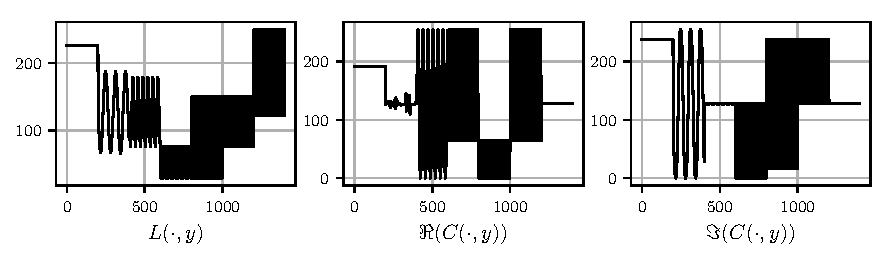
\includegraphics[width=\textwidth]{horizontal_line_three_channel_decomposition.pdf}}    
\caption{Illustration of the proposed synthetic image: (a) Luminance and chrominance decomposition; (b) Horizontal line trough the three channels.}\label{fig:three_channel_decomposition}
\end{figure}

\section{Gabor feature space validation}
The feature space calculated from the spectral decomposition of the image captures the color and texture information generated by changes in color and lighting in the image. To visually validate the quality of the feature space, we implement three clustering methods. In addition, we also propose a set of high-level features based on Gabor energy recovered from the real and complex channels of the image.

\subsection{Clustering methods as a technique for color image segmentation}


\subsubsection{k-means clustering}
\subsubsection{Gaussian mixture clustering}
\subsubsection{Birch clustering}





\section{Conclusion}
